\documentclass[t]{sdqbeamer}
%\documentclass[c]{sdqbeamer}

\usepackage{listings}
\usepackage{graphicx}
\usepackage{tabularx}

% set sdqbeamer options
\titleimage{BoolCircuit}
\groupname{Algorithm Engineering}
\grouplogo{ae_cycle}
\selectlanguage{english}

% define title etc.pp.
\title[SAT Solving]{Practical SAT Solving}
\subtitle{Lecture 1}
\author{\underline{Markus Iser}, Dominik Schreiber, Tom\'a\v{s} Balyo}
\date{April 15, 2024}

% Existing KIT colors: kit-green, kit-blue, kit-red, kit-gray, kit-orange, kit-lightgreen, kit-brown, kit-purple, kit-cyan
% configure appearance
\setbeamercolor{block title}{bg=kit-blue}
\setbeamercolor{block body}{bg=kit-blue!10}
\setbeamercolor{block title example}{bg=kit-orange}
\setbeamercolor{block body example}{bg=kit-orange!10}
\setbeamertemplate{itemize item}{\color{kit-gray}\textbullet}
\setbeamertemplate{itemize subitem}{\color{kit-gray}\textbullet}
\setbeamercolor{item projected}{bg=kit-gray, fg=kit-gray}
\renewcommand{\insertnavigation}[1]{} % remove navigation bar

% define commands
\definecolor{myblue}{HTML}{0D3B66}
\definecolor{myred}{HTML}{6E0E0A}
\definecolor{mypink}{HTML}{F7B2B7}

\newcommand{\vars}[1]{\textsf{vars} (#1)}
\newcommand{\lits}[1]{\textsf{lits} (#1)}
\newcommand{\clss}[1]{\textsf{clss} (#1)}

\newcommand{\highl}[1]{\textcolor{myblue}{#1}}
\newcommand{\highlo}[1]{\textcolor{myred}{#1}}
\newcommand{\highlow}[1]{\textcolor{mypink}{#1}}

% Extra column types for tabularx
\newcolumntype{C}{>{\centering\arraybackslash}X}
\newcolumntype{L}{>{\raggedright\arraybackslash}X}
\newcolumntype{R}{>{\raggedleft\arraybackslash}X}

\newcommand{\setcolsep}[1]{\setlength{\tabcolsep}{#1}}
\newcommand{\setrowsep}[1]{\renewcommand{\arraystretch}{#1}}

% Definitions for the Tseitin transformation
\newcommand{\true}{\ensuremath{\mathit{True}}}
\newcommand{\false}{\ensuremath{\mathit{False}}}
\newcommand{\allvars}{\ensuremath{\mathcal{V}}}
\newcommand{\tseitin}[1]{\ensuremath{\mathcal{T}(#1)}}
\newcommand{\tseitinRec}[2]{\ensuremath{\mathcal{T}^{#2}(#1)}}
\newcommand{\tseitinSym}[1]{\ensuremath{\mathcal{T}_\mathsf{lit}(#1)}}
\newcommand{\tseitinDef}[2]{\ensuremath{\mathcal{T}_\mathsf{def}^{#2}(#1)}}
\newcommand{\hcancel}[2][black]{\setbox0=\hbox{$#2$}\rlap{\raisebox{.45\ht0}{\textcolor{#1}{\rule{\wd0}{1pt}}}}#2} 
\newcommand{\sateq}{\mathrel{\overset{\makebox[0pt]{\mbox{\normalfont\tiny\sffamily SAT}}}{=}}}

\newcommand{\enc}{\ensuremath{\mathcal{E}}} % encoding

% exercise commands
\newcommand{\exhead}[3]{
\hrule~\\[1ex]\noindent
{\bf Practical SAT Solving} (ST 2024) \hfill \fbox{Assignment #1} \\[1ex]
Markus Iser, Dominik Schreiber, Tom\'a\v{s} Balyo\\[1ex]
Algorithm Engineering (KIT) \hfill #2 -- #3\\
\hrule
\thispagestyle{empty}
}


\begin{document}

\begin{frame}
	\thispagestyle{empty}
	\titlepage
\end{frame}

\section{Organisational}
\begin{frame}{Organisation}
	\begin{itemize}\setlength{\itemsep}{1em}
		\item 14 Lectures: Mondays at 3:45 pm, room 301 (starting today)
		\item 6 Exercises: Tuesdays at 3:45 pm, room 301 (starting 4/23, every other week!)
		\item Bring your laptop if you can!
		\item Sign up:
		\begin{itemize}
			\item \url{http://campus.studium.kit.edu}
		\end{itemize}
		\item Find material (slides, exercises, etc.):
		\begin{itemize}
			\item \url{https://github.com/satlecture/kit2024}
		\end{itemize}
		% \item Interact with us (feedback, questions, announcements, etc.):
		% \begin{itemize}
		% 	\item \url{https://ilias.studium.kit.edu}
		% \end{itemize}
	\end{itemize}
\end{frame}

\begin{frame}{Lecturers}
\begin{itemize}\setlength{\itemsep}{1em}
	\item Markus Iser, \href{mailto:markus.iser@kit.edu}{markus.iser@kit.edu}
	\begin{itemize}
		\item post-doc at ITI Sanders, involved in this lecture since 2020
		\item expert on SAT solvers and benchmarks
	\end{itemize}
	\item Dominik Schreiber, \href{mailto:dominik.schreiber}{dominik.schreiber@kit.edu}
	\begin{itemize}
		\item post-doc at ITI Sanders, involved in this lecture since 2023
		\item expert on massively parallel SAT solving
	\end{itemize}
	\item Tom\'a\v{s} Balyo, \href{mailto:tomas@filuta.ai}{tomas@filuta.ai}
	\begin{itemize}
		\item previously post-doc at ITI Sanders, started this lecture in 2016 with Carsten Sinz
		\item now research engineer at a composite AI start-up
		\item will offer some guest lectures 
	\end{itemize}
\end{itemize}
\end{frame}

\begin{frame}{Homework, Competitions, and Oral Exam}
\begin{itemize}\setlength{\itemsep}{1em}
	\item You earn exercise points for doing homework and coming to class with your solutions.
	\item You can earn at least 120 exercise points during the semester (plus many more bonus points).
	\begin{itemize}
		\item Some exercises will be in the form of small implementation contests.
		\item Contest winners will receive bonus points.
	\end{itemize}
	\item You must earn at least 60 points to participate in the oral exam.
	\item Bonus points for homework will improve your grade.
\end{itemize}
\end{frame}

\begin{frame}{Goals of this Lecture}
\begin{block}{Efficient Methods for SAT Solving}
	Algorithms, Heuristics, Data Structures, Implementation Techniques, Parallelism, Proof Systems, \dots
\end{block}
\pause
\begin{block}{Applications of SAT Solving}
	Verification of Hardware and Software, Planning, Scheduling, Cryptography, Explainable AI, \dots
\end{block}
\pause
\begin{block}{Efficient Encodings of Problems into SAT}
	General Encoding Techniques, CNF Encodings of Constraints, Properties of CNF Encodings, \dots
\end{block}
\pause
\begin{block}{Practical Hardness of SAT}
	Tractable Classes, Instance Structure, Hardest Instances, Proof Complexity, \dots
\end{block}
\end{frame}


\section{Basic Definitions}

\begin{frame}{Basic Definitions}

In this lecture, propositional formulas are given in \emph{conjunctive normal form} (CNF), and if not, we convert them.

\begin{block}{CNF Formulas}
	\begin{itemize}
		\item A \emph{CNF formula} is a conjunction (and = $\wedge$) of clauses.
		\item A \emph{clause} is a disjunction (or = $\vee$) of literals.
		\item A \emph{literal} is a Boolean variable $x$ (positive literal) or its negation $\overline{x}$ (negative literal).
	\end{itemize}	
\end{block}

\begin{example}[CNF Formula]
	\vspace{-3ex}
	\begin{align*}
		F &= (\overline{x_1} \vee x_2) \wedge (\overline{x_1} \vee \overline {x_2} \vee x_3) \wedge (x_1)\\
		\vars{F} &= \{x_1, x_2, x_3\}\\
		\lits{F} &= \{x_1, \overline{x_1}, x_2, \overline{x_2}, x_3\}\\
		\clss{F} &= \{ \{ \overline{x_1}, x_2 \}, \{ \overline{x_1}, \overline {x_2}, x_3 \}, \{ x_1 \} \}
	\end{align*}
	Typically, a CNF formula is given as a set of clauses, where each clause is a set of literals (as in $\clss{F}$).
\end{example}
\end{frame}

\begin{frame}{Satisfiability}
	The \emph{Satisfiability Problem} is to determine whether a given formula is satisfiable.\\
	A CNF formula $F$ is \emph{satisfiable} iff there exists an assignment to $\vars{F}$ that satisfies $F$.
	\begin{block}{Satisfying Assignment}
		Given a CNF formula $F$ over variables $V := \vars{F}$, a \emph{truth assignment} $\phi : V \rightarrow \{ \top, \bot \}$ assigns a truth value $\top$ (True) or $\bot$ (False) to each Boolean variable in $V$.\\[1em]
		We say that $\phi$ satisfies
			\begin{itemize}
				\item a CNF formula if it satisfies all of its clauses
				\item a clause if it satisfies at least one of its literals
				\item a positive literal $x$ if $\phi(x)=\top$
				\item a negative literal $\overline{x}$ if $\phi(x)=\bot$
			\end{itemize}
	\end{block}
\end{frame}

\begin{frame}{Satisfiability}
\begin{example}[Satisfiable or Unsatisfiable?]
	\vspace*{-3ex}
	\begin{align*}
		F_1 &= \{ \{ x_1 \} \}\\[1ex]
		F_2 &= \{ \{ x_1 \}, \{ \overline{x_1} \} \}\\[1ex]
		F_3 &= \{ \{ x_2, x_8, \overline{x_3} \} \}\\[1ex]
		F_4 &= \{ \{ x_1 \}, \{ \overline{x_2} \}, \{ x_2, \overline{x_1} \} \}\\[1ex]
		F_5 &= \{ \{ x_1, x_2 \}, \{ \overline{x_1}, x_2 \}, \{ x_1, \overline{x_2} \}, \{ \overline{x_1}, \overline{x_2} \} \}\\[1ex]
		F_6 &= \{ \{ \overline{x_1}, x_2 \}, \{ \overline{x_1}, \overline {x_2}, x_3 \}, \{ x_1 \} \}
	\end{align*}
\end{example}
\pause
\begin{alert}{Edge Cases:\\}
	What are the shortest satisfiable / unsatisfiable CNF formulas?
\end{alert}
\end{frame}

\begin{frame}{Satisfiability}
	\begin{example}[Scheduling]
		Schedule a meeting of Adam, Bridget, Charles, and Darren considering the following constraints
		\begin{itemize}
			\item Adam can only meet on Monday or Wednesday
			\item Bridget cannot meet on Wednesday
			\item Charles cannot meet on Friday
			\item Darren can only meet on Thursday or Friday
		\end{itemize}
		\vspace*{-2ex}
		\begin{align*}
			\vars{F} &= \{ x_1, x_2, x_3, x_4, x_5 \}\\
			F &= 
			\visible<2->{(x_1 \vee x_3) \wedge (\overline{x_3}) \wedge (\overline{x_5}) \wedge (x_4 \vee x_5)\\}
			\only<3>{&\wedge \operatorname{AtMostOne}(x_1, x_2, x_3, x_4, x_5) \\}
			\only<4>{
				&\wedge (\overline{x_1} \vee \overline{x_2}) \wedge (\overline{x_1} \vee \overline{x_3}) \wedge (\overline{x_1} \vee \overline{x_4}) \wedge (\overline{x_1} \vee \overline{x_5})\\
				&\wedge (\overline{x_2} \vee \overline{x_3}) \wedge (\overline{x_2} \vee \overline{x_4}) \wedge (\overline{x_2} \vee \overline{x_5})\\
				&\wedge (\overline{x_3} \vee \overline{x_4}) \wedge (\overline{x_3} \vee \overline{x_5}) \wedge (\overline{x_4} \vee \overline{x_5})
			}
		\end{align*}
	\end{example}
	\only<4>{Is this Scheduling Instance Satisfiable?}
\end{frame}

\begin{frame}{Complexity of Propositional Satisfiability}
\vspace*{-1em}
A decision problem is NP-complete if it is in NP and every problem in NP can be reduced to it in polynomial time.
\begin{block}{SAT is NP-complete (Cook-Levin Theorem)}
\begin{itemize}\setlength{\itemsep}{.5ex}
	\item SAT is in NP\\
	\textbf{Proof:} solution can be checked in polynomial time
	\item Every problem in NP can be reduced to SAT in polynomial time\\
	\textbf{Proof:} encode the run of a non-deterministic Turing machine as a CNF formula
\end{itemize}
\end{block}
\pause
\begin{block}{Consequences of NP-completeness of SAT}
\begin{itemize}
	\item We do not have a polynomial algorithm for SAT (yet) :(
	\item If $P \neq NP$ then we will never have a polynomial algorithm for SAT :'(
	\item All the known NP-complete algorithms have exponential runtime in the \textbf{worst case}.
\end{itemize}
\end{block}

\begin{example}[Hardness]
Try it yourself: \url{http://www.cs.utexas.edu/~marijn/game/}
\end{example}
\end{frame}

\begin{frame}{History of Propositional Satisfiability}
\begin{block}{Historic Landmarks}
	\begin{itemize}\setlength{\itemsep}{1ex}
		\item \href{http://doi.acm.org/10.1145/321033.321034}{1960: DP Algorithm (first SAT solving algorithm)}
		% Davis, Putnam: A Computing Procedure for Quantification Theory
		\item \href{https://doi.acm.org/10.1145/368273.368557}{1962: DPLL Algorithm (improving upon DP algorithm)}
		% Davis, Logemann, Loveland: A Machine Program for Theorem-Proving
		\item \href{https://dl.acm.org/doi/10.1145/800157.805047}{1971: SAT is NP-Complete}
		% Cook: The Complexity of Theorem-Proving Procedures
		\item \href{http://www.aaai.org/Library/AAAI/1992/aaai92-068.php}{1992: Local Search Algorithm}
		Selman et al.: A New Method for Solving Hard Satisfiability Problems
		\item 1992: The First International SAT Competition (followed by 1993, 1996, since 2002 every year)
		\item 1996: The First International SAT Conference (Workshop) (followed by 1998, since 2000 every year)
		\item \href{https://doi.org/10.1109/12.769433}{1999: Conflict Driven Clause Learning (CDCL) Algorithm}
		% Marques-Silva, Sakallah: GRASP: A Search Algorithm for Propositional Satisfiability
	\end{itemize}
\end{block}
\begin{alert}{Advancements}
	From 1992 to 2024, SAT solvers have improved by several orders of magnitude in terms of feasible problem size.
	From 100 variables and 200 clauses to 21,000,000 variables and 96,000,000 clauses.
\end{alert}
\end{frame}

\begin{frame}{SAT Conference 2022}
	\centering
	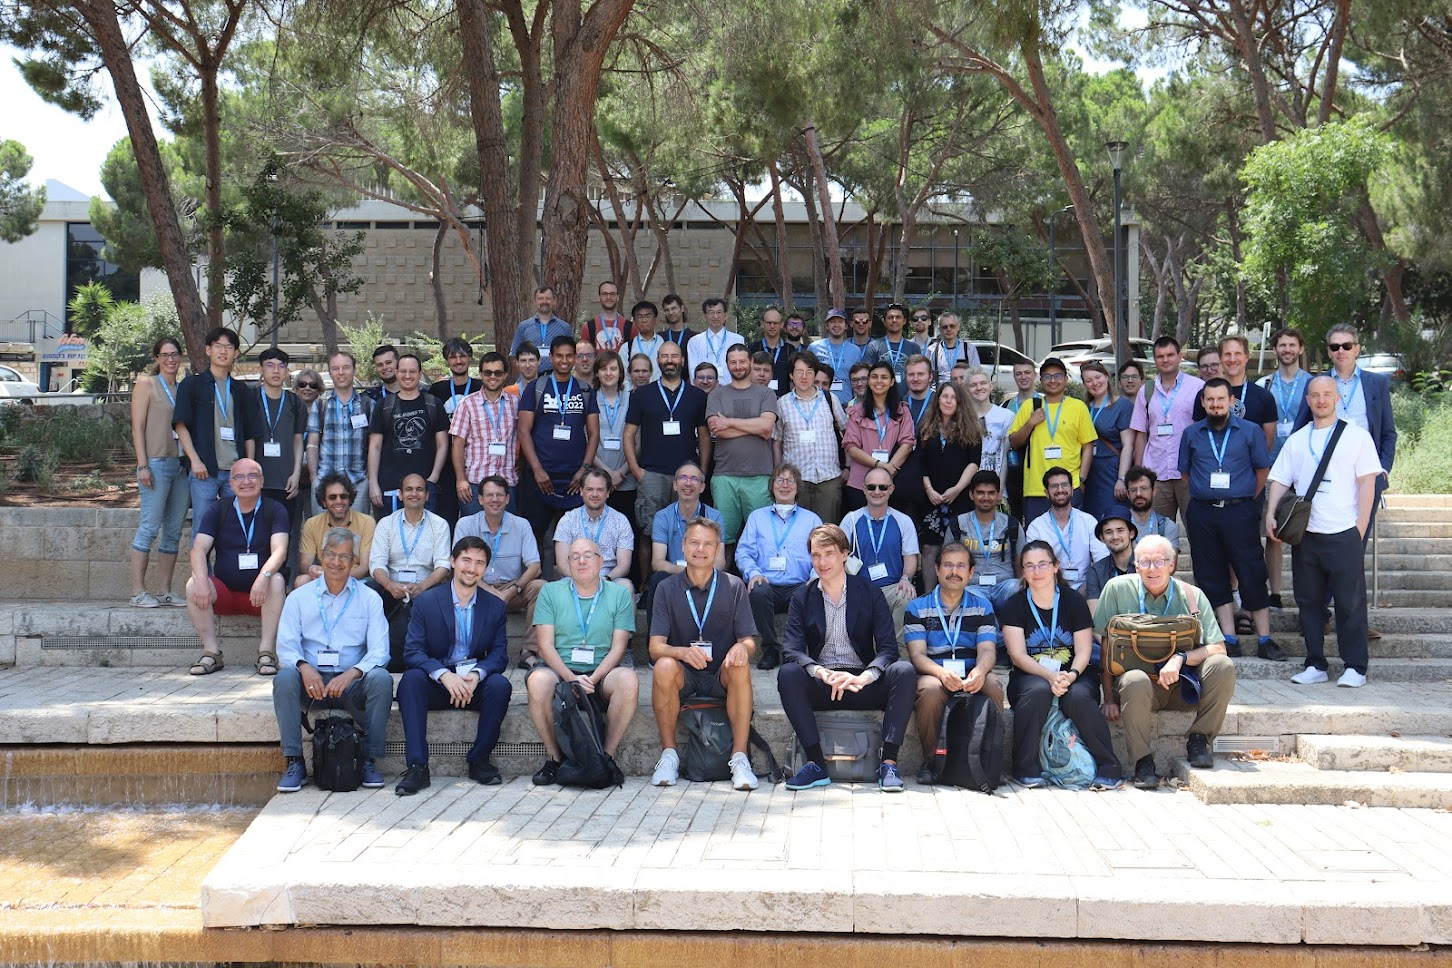
\includegraphics[height=.75\textheight]{figures/l01/SAT2022-grouppicture.jpg}
\end{frame}

\section{Introductory Examples}

\begin{frame}{Applications of SAT Solving}
\begin{minipage}{0.75\textwidth}
	\begin{itemize}
		\item Hardware verification and design
		\begin{itemize}
			\item Major hardware companies (Intel, \dots) use SAT to verify their chip designs
			\item Computer Aided Design of electronic circuits
		\end{itemize}
		\item Software verification
		\begin{itemize}
			\item SAT-based SMT solvers are used to verify Microsoft software products\\
			(also great interest at Amazon -- AWS software in particular)
			\item Embedded software in cars, airplanes, refrigerators,~\dots
			\item Unix utilities
		\end{itemize}
		\item Automated Planning and Scheduling in Artificial Intelligence
		\begin{itemize}
			%\item Good for small-to-medium sized, highly constrained problems
			\item Job shop scheduling, train scheduling, multi-agent path finding
		\end{itemize}
		\item Cryptanalysis
		\begin{itemize}
			\item Test/prove properties of cryptographic ciphers, hash functions
		\end{itemize}
		\item Number Theoretic Problems (Pythagorean Triples, square grid coloring)
		\item Solving other NP-hard problems (coloring, clique, \dots)
	\end{itemize}	
\end{minipage}%
\begin{minipage}{0.25\textwidth}
	
\includegraphics[width=\textwidth]{figures/l01/applications.png}
\end{minipage}
\end{frame}

\begin{frame}{SAT Solving in the News}
	\centering
	
\includegraphics[height=.75\textheight]{figures/l01/triples-spiegel.png}
\end{frame}

\begin{frame}{Pythagorean Triples}
\begin{block}{Problem Definition}
Is it possible to assign to each integer $1,2,\ldots,n$ one of two colors such that if
$a^2+b^2=c^2$ then $a,b$ and $c$ do not all have the same color.
\end{block}
\begin{itemize}
	\item Solution: Nope
	\item for $n=7825$ it is not possible
	\item proof obtained by a SAT solver has 200 Terrabytes -- the largest Math proof ever
\end{itemize}
\pause
\begin{block}{How to encode this?}
\begin{itemize}
	\item for each integer $i$ we have a Boolean variable $x_i$, $x_i=1$ if color of $i$ is 1, $x_i=0$ otherwise.
	\item for each $a,b,c$ such that $a^2+b^2=c^2$ we have two clauses: $(x_a \vee x_b \vee x_c)$
	and $(\overline{x_a} \vee \overline{x_b} \vee \overline{x_c})$
\end{itemize}
\end{block}
\end{frame}


\begin{frame}{Arithmetic Progressions}
\begin{block}{Problem Definition}
	Find a binary sequence $x_1, \dots, x_n$ that has no $k$ equally spaced 0s and no $k$ equally spaced 1s.
\end{block}
\pause
\begin{example}[$n=8, k=3$]
Find a binary sequence $x_1,\dots,x_8$ that has no three equally spaced 0s and no three equally spaced 1s.
\begin{itemize}
\item<2-> What about 01001011? \uncover<3->{No, the 1s at $x_2, x_5, x_8$ are equally spaced.}
\item<4-> 6 Solutions: 00110011, 01011010, 01100110, 10011001, 10100101, 11001100.
\item<5-> Extending the problem to 9 digits, no solutions remains. How can we show this with a SAT solver?
\item<6-> Encode what's forbidden: $x_2 x_5 x_8 \neq 111$ is the same as
   $(\overline{x_2} \lor \overline{x_5} \lor \overline{x_8})$.
\item<7-> Writing, e.g., $\bar 2 \bar 5 \bar 8$ for the clause $(\overline{x_2} \lor \overline{x_5} \lor \overline{x_8})$, we arrive
  at 32 clauses for the 9 digit sequence: \\
  $123, 234, \dots, 789, 135, 246, \dots, 579, 147, 258, 369, 159$,
  $\bar 1 \bar 2 \bar 3, \bar 2 \bar 3 \bar 4, \dots, \bar 7 \bar 8 \bar 9, \bar 1 \bar 3 \bar 5, \bar 2 \bar 4 \bar 6, 
  \dots, \bar 5 \bar 7 \bar 9, \bar 1 \bar 4 \bar 7, \bar 2 \bar 5 \bar 8, \bar 3 \bar 6 \bar 9, \bar 1 \bar 5 \bar 9$.
\end{itemize}
\end{example}
\end{frame}

\begin{frame}{Background: Van der Waerden Numbers}
\begin{block}{Theorem (van der Waerden)}
If $n$ is sufficiently large, every sequence $x_1, \dots, x_n$ of numbers $0 \leq x_i < r$ contains a number that occurs at least $k$ times equally spaced.
\begin{itemize}
\item The smallest such number is the van der Waerden number $W(r,k)$.
\item For larger $r, k$ the numbers are only partially known.
\end{itemize}
\end{block}
\pause
\begin{example}[Van der Waerden Numbers]
\begin{itemize}
	\item We have seen that $W(2,3) = 9$.
	\item $W(2,6) = 1132$ was shown in \href{http://dx.doi.org/10.1080/10586458.2008.10129025}{[2008 by Kouril and Paul]} (using a SAT solver!)
	\item but $W(2,7)$ is yet unknown.
	\item $2^{2^{r^{2^{2^{k+9}}}}}$ is an upper bound for $W(r,k)$ (shown in \href{http://dx.doi.org/10.1007/s00039-001-0332-9}{[2001 by Gowers]}).
\end{itemize}
\end{example}
\end{frame}

\begin{frame}{Graph Coloring}
\begin{example}[McGregor Graph, 110 nodes, planar]
	Claim: Cannot be colored with less than 5 colors. (Scientific American, 1975, Martin Gardner's column ``Mathematical Games'')
	\begin{center}
		\includegraphics<1>[height=4.5cm]{figures/l01/macgregor-bw.jpg}
		\includegraphics<2>[height=4.5cm]{figures/l01/macgregor_arb.jpg}
	\end{center}
\end{example}
\end{frame}

\begin{frame}{Graph Coloring: SAT Encoding}
\begin{block}{Definition: Graph Coloring Problem (GCP)}
Given an undirected graph $G=(V,E)$ and a number $k$, a $k$-coloring assigns one of $k$ colors to each node, such that all adjacent nodes have a different color. The GCP asks whether a $k$-coloring for $G$ exists.
\end{block}
\pause
\begin{alert}{SAT Encoding}
\begin{itemize}
\item<2-> Variables: 
\begin{itemize}
	\item<3-> use $k \cdot |V|$ Boolean variables $v_j$ for $v \in V$, where $v_j$ is true, if node $v$ gets color $j$ ~($1 \leq j \leq k$).
\end{itemize}
\item<3-> Clauses: 
\begin{itemize}\setlength{\itemsep}{.5ex}
	\item<4-> Every node gets a color: 
	\item[]<5-> \quad $(v_1 \lor \cdots \lor v_k)\,$ for $v \in V$
	\item<6-> Adjacent nodes have different colors: 
	\item[]<7-> \quad $(\overline{u_j} \lor \overline{v_j})\,$ for ${u,v} \in E, 1 \leq j \leq k$
	\item<8-> Suppress multiple colors for a node: At-most-one constraints
\end{itemize}
\end{itemize}
\end{alert}
\end{frame}

\begin{frame}{Graph Coloring: Example}
\begin{example}[Graph Coloring Problem]
\begin{columns}
	\begin{column}{0.6\textwidth}
	\begin{itemize}
	\item $V = \{ u, v, w, x, y \}$
	\item Colors: red (=1), green (=2), blue (=3)
	\item Clauses: \\
	\textcolor{gray}{``every node gets a color''} \\
	$(u_1 \lor u_2 \lor u_3)$ \\
	$\quad\vdots$ \\ 
	$(y_1 \lor y_2 \lor y_3)$ \\ \vspace{0.5ex}
	\textcolor{gray}{``adjacent nodes have different colors''}
	$(\overline{u_1} \lor \overline{v_1}) \land \cdots \land (\overline{u_3} \lor \overline{v_3})$ \\
	$\quad\vdots$ \\
	$(\overline{x_1} \lor \overline{y_1}) \land \cdots \land (\overline{x_3} \lor \overline{y_3})$
	\end{itemize}
	\end{column}
	\begin{column}{0.4\textwidth}
	\begin{center}
		\includegraphics<1>[height=0.7\textwidth]{figures/l01/graph-coloring-1.pdf}
		\includegraphics<2>[height=0.7\textwidth]{figures/l01/graph-coloring-2.pdf}
	\end{center}
	\end{column}
\end{columns}
\end{example}
\end{frame}

\begin{frame}{Using a SAT Solver}
SAT solvers are command line applications that take as argument a text file with a formula (DIMACS format).
\begin{example}[Input]
	\texttt{c comments, ignored by solver}\\
	\texttt{p cnf 7 22}\\
	\texttt{1 -2 7 0}\\
	\texttt{...}\\
	\texttt{-7 -3 -2 0}
\end{example}
\pause
\begin{example}[Output]
	\texttt{c comments, usually some stastitics about the solving}\\
	\texttt{s SATISFIABLE} \hspace{4em}\\
	\texttt{v 1 2 -3 -4}\\
	\texttt{v 5 -6 -7 0}\\
\end{example}
\end{frame}

\begin{frame}{Running a SAT Solver}
\begin{alert}{Let's try it!}
	\begin{itemize}\setlength{\itemsep}{1em}
		\item Download and Build a SAT solver:
			\begin{itemize}
				\item \href{https://github.com/arminbiere/cadical}{CaDiCaL}
				\item Alternatives: \href{https://github.com/arminbiere/kissat}{Kissat}, \href{https://github.com/niklasso/minisat}{Minisat}, \href{https://github.com/msoos/cryptominisat}{CryptoMinisat}, \href{https://maplesat.github.io/}{Maplesat}, \dots
			\end{itemize}
		\item Download a CNF formula:
			\begin{itemize}
				\item \href{https://benchmark-database.de}{Global Benchmark Database}
			\end{itemize}
		\item Run the SAT solver with the CNF formula as input
	\end{itemize}
\end{alert}
\end{frame}


\section{Incremental SAT}

\begin{frame}{Incremental SAT Solving}
In many applications, we solve a sequence of similar SAT instances:\\[1ex]
Planning, Bounded Model Checking, SMT, Scheduling, MaxSAT, \dots

\begin{block}{Incremental SAT Solving}
\begin{itemize}\setlength{\itemsep}{1em}
	\item The SAT solver is initialized once
	\item Each call to \texttt{solve()} takes a set of assumptions as input\\
		  $\rightarrow$ assumptions are literals that serve as a partial assignment to their variables
	\item Like this also clauses can be activated/deactivated in the SAT solver
	\item Between \texttt{solve()} calls, new clauses can be added
	\item Advantages:
	\begin{itemize}
		\item<2-> solver remembers learned clauses, preprocessing, variable scores (heuristics), etc.
		\item<2-> (de)initialization overheads removed
	\end{itemize}
\end{itemize}
\end{block}
\end{frame}

\begin{frame}{IPASIR: Incremental Library Interface for SAT Solvers}
IPASIR = Re-entrant Incremental Satisfiability Application Program Interface (acronym reversed)

\begin{block}{IPASIR}
	\begin{itemize}\setlength{\itemsep}{1em}
		\item Defined for the 2015 SAT Race to unify incremental SAT solver interfaces
		\item IPASIR has become a standard interface of incremental SAT solving
		\item<2> Version 2 is in the works
	\end{itemize}
\end{block}~\\[.5em]
\centering
% \only<1>{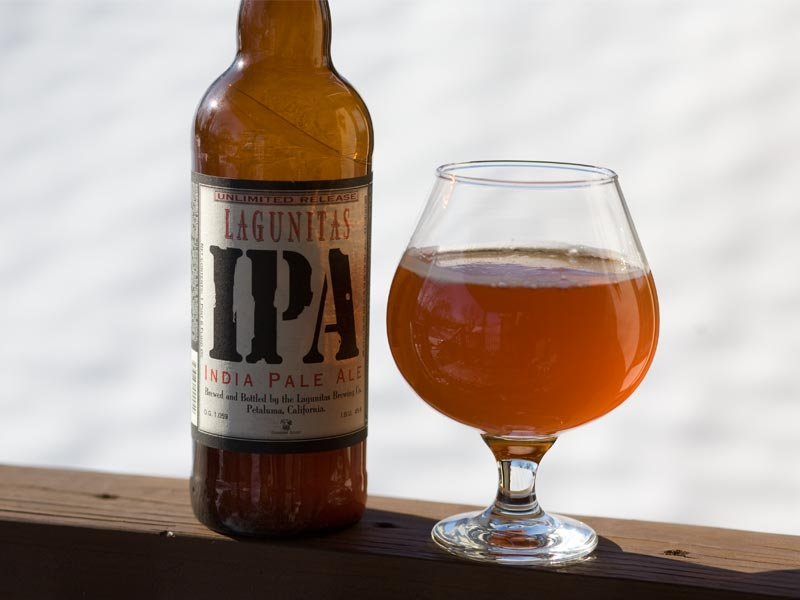
\includegraphics[width=.23\textwidth]{figures/l01/ipa.jpeg}}
\only<1>{\href{https://github.com/biotomas/ipasir}{
\includegraphics[width=.23\textwidth]{logos/ipasir.png}}}
\only<2>{\href{https://github.com/ipasir2}{
\includegraphics[width=.23\textwidth]{logos/ipasir2.png}}}
\end{frame}

\begin{frame}{IPASIR Overview}
\begin{itemize}
\item Clauses are added one literal at a time
\begin{itemize}
	\item To add $(x_1 \vee \overline{x_4})$ call \texttt{add(1); add(-4); add(0);}
\end{itemize}
\item You can call a SAT solver with a set of assumptions
\begin{itemize}
	\item Assumptions are basically temporary decision literals
	\item Assumptions are cleared after each \texttt{solve()} call
\end{itemize}
\item Clause removal is done via activation literals and assumptions
\begin{itemize}
	\item You must know ahead which clauses you will maybe want to remove
	\item Add the clause with an additional fresh variable (activation literal)
	\item example: instead of $(x_1 \vee x_2)$ add $(x_1 \vee x_2 \vee a_1)$
	\item solve with with assumption $\overline{a_1}$ to enforce $(x_1 \vee x_2)$
	\item drop the assumption $\overline{a_1}$ to drop $(x_1 \vee x_2)$
\end{itemize}
\end{itemize}
\end{frame}

% \begin{frame}{Ipasir Interface}
% \begin{block}{ipasir.h}
% \texttt{\footnotesize
% const char* ipasir\_signature();\\
% void* ipasir\_init();\\
% void  ipasir\_release(void* solver);\\
% void  ipasir\_set\_terminate(void* solver, void* state,\\
% \hspace{2em} int (*terminate)(void* state));\\
% void  ipasir\_set\_learn (void * solver, void * state,\\
% \hspace{2em} int max\_length, void (*learn)(void * state, int * clause));\\
% void  ipasir\_add(void* solver, int lit\_or\_zero);\\
% void  ipasir\_assume(void* solver, int lit);\\
% int   ipasir\_solve(void* solver);\\
% int   ipasir\_val(void* solver, int lit);\\
% int   ipasir\_failed(void* solver, int lit);
% }
% \end{block}
% \end{frame}

\begin{frame}{IPASIR Functions}
	\def\arraystretch{1.5}
	\begin{tabularx}{\textwidth}{lX}
		\tt signature 	& return the name and version of the solver\\
		\tt init    	& initialize the solver, the pointer it returns is used for the rest of the functions\\
		\tt add 		& add clauses, one literal at a time\\
		\tt assume 		& add an assumption, the assumptions are cleared after a "solve" call\\
		\tt solve 		& solve the formula, return SAT, UNSAT or INTERRUPTED\\
		\tt val 		& return the truth value of a variable (if SAT)\\
		\tt failed 		& returns true if the given assumption was part of reason for UNSAT\\
	\end{tabularx}~\\[1em]
	For more details and examples of usage see \url{https://github.com/biotomas/ipasir}
\end{frame}

\begin{frame}{IPASIR Solver States}
\centering
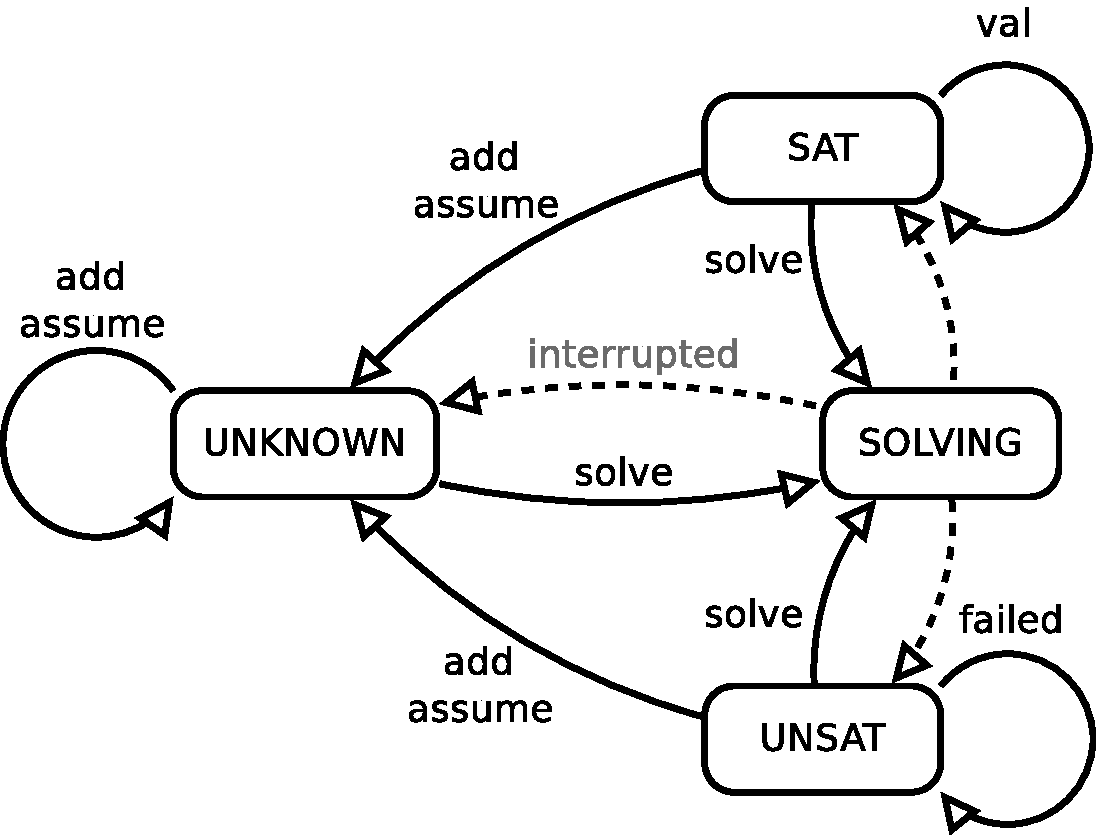
\includegraphics[height=.75\textheight]{figures/l01/ipasir.pdf}
\end{frame}

\begin{frame}{Use Case: Essential Variables}
Let a satisfiable formula $F$ be given.
\begin{block}{Essential Variables}
\begin{itemize}\setlength{\itemsep}{1em}
	\item Satifying assignments can be partial, i.e., some variables are not assigned but still the formula is satisfied.
	\item A variable $x$ is \emph{essential} if and only $x$ it has to be assigned (True or False) in each satisfying assignment.
\end{itemize}
\end{block}
\begin{block}{Task: find all the essential variables of a given satisfiable formula}
	\begin{itemize}\setlength{\itemsep}{1ex}
		\item use \emph{Dual Rail Encoding} -- for each variable $x$ add two new variables $x_P$ and $x_N$,
		replace each positive (negative) occurrence of $x$ with $x_P$ ($x_N$), add a clause
		$(\overline{x_P} \vee \overline{x_N})$ (meaning $x$ cannot be both true and false).
		\item for each variable $x$ solve the formula with the assumptions $\overline{x_P}$ and
		$\overline{x_N}$. If the formula is UNSAT then $x$ is essential.
	\end{itemize}
\end{block}
\begin{alert}{Let's implement it!}
	\href{https://github.com/satlecture/kit2024/tree/main/code}{https://github.com/satlecture/kit2024/tree/main/code}
\end{alert}
\end{frame}

% \begin{frame}{Example -- Essential Variables -- Code}
% 	\centering
% 	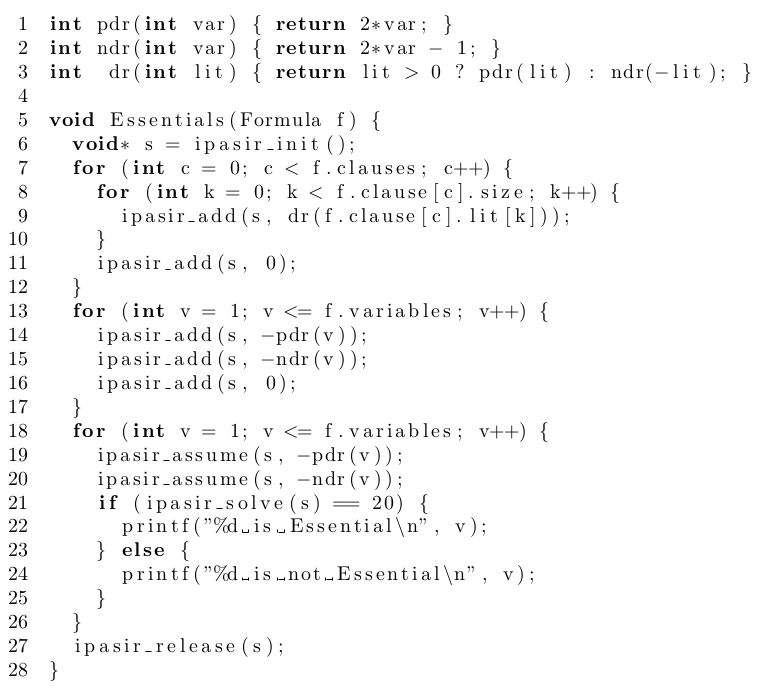
\includegraphics[height=.75\textheight]{figures/l01/essentials.png}
% \end{frame}

% \appendix
% \beginbackup

% \begin{frame}[allowframebreaks]{References}
% \bibliographystyle{templates/bibstyle}
% \bibliography{references}
% \end{frame}

% \backupend

\end{document}
